\documentclass[10pt,a4paper]{article}
\usepackage[margin=2cm]{geometry}
\usepackage{amsmath,amssymb,booktabs,graphicx,caption,xcolor,float,hyperref,tikz}
\usetikzlibrary{arrows.meta,positioning,calc}
\hypersetup{colorlinks=true,linkcolor=blue!50!black,urlcolor=blue!50!black}
\captionsetup{font=small,labelfont=bf}
\title{\vspace{-1.2cm}\textbf{Steering a swarm that owns a proof}\\[2pt]
\large Simulation 1 (days and nights), setup \texttt{task003-symmetric}}
\author{LLM-free simulator; report of 16 October 2026; runs of 15 October 2026\\
\small Mirrors the Simulation 2 report of the same date: same sections, figures and equations. Same data as the 15 October version, reorganised.}
\date{}
\begin{document}
\maketitle
\vspace{-1cm}

\paragraph{How the simulator works.} The world, \texttt{task\_003}, has three candidate allocations; A0 is the
correct one. Each of 24 agents is given one true fact and reasons as an exact Bayesian: its \emph{belief} is the
exact probability of A0, A1 and A2 given the facts it currently remembers. An episode has 30 rounds, each a day
and a night. During the day the agents act one at a time in a new random order: an agent reads $q$ posts drawn at
random from a shared \emph{board} (never its own), adds their facts to its memory, recomputes its belief,
\emph{votes} by probability matching (a vote drawn from its belief) and posts one remembered fact that supports
its vote. At night a \emph{controller} with a target, A0 (truth) or A2 (false), reads $q_c$ agent posts and,
unless the \emph{vote gate} (at least 75\% of them from agents voting for its target) or the \emph{proof stop}
(what it read already proves its target) silences it, posts the $b$ facts from its pool that best support its
target. The board is then cleared, keeping only the controller's new posts. At each dawn every remembered fact is
forgotten with probability $1-\rho$ and comes back if read again. Every episode is run three times with the same
random draws: without a controller (\emph{silent}), with the controller targeting A0 and with the one targeting
A2.

\paragraph{The facts at the start.} All facts are true. The agents hold, together, a proof of A0; no single
agent does, and neither pool can prove its target (Table~\ref{tab:facts}).

\begin{table}[H]
\centering\small
\caption{Facts available at the start and what each set implies, $P(\text{A0}, \text{A1}, \text{A2} \mid \text{facts})$.}
\label{tab:facts}
\begin{tabular}{lcc}
\toprule
set of facts & facts & $P(\text{A0}, \text{A1}, \text{A2})$ \\
\midrule
agents' facts, all together (24 agents, one fact each) & 18 distinct & (1, 0, 0): proves A0 \\
A0 pool (controller with target A0) & 12, of which 10 new to the agents & (0.963, 0.037, 0) \\
A2 pool (controller with target A2) & 12, of which 10 new to the agents & (0.114, 0, 0.886) \\
agents' facts + either pool & 28 distinct & (1, 0, 0) \\
\bottomrule
\end{tabular}
\end{table}

\paragraph{The runs.} Posts read by an agent $q \in \{3, 6, 12\}$; posts read by the controller
$q_c \in \{3, 6, 12, 24\}$; facts posted per night $b \in \{1, \dots, 9\}$ (at most 12, the pool size); memory
$\rho \in \{1, 0.75, 0.5, 0.25\}$; vote gate on and off; proof stop on; 1{,}000 episodes per setting (1{,}740
settings). Unless stated otherwise: $q = 6$, $q_c = 12$, $b = 1$ (the main setting, which posts about as many
facts as Simulation 2 at rate 1), gate on. The vote gate is on throughout.

\paragraph{Summary.} The 24 agents together own a proof of A0, and with full memory they keep it: no controller
changes the swarm for more than a few days. \textbf{Forgetting is what makes the swarm steerable}, and in this
simulation the effect peaks at intermediate memory: at $\rho = 0.5$ the false controller wins 78\% of the votes
(Figure~\ref{fig:votes}). Seen side by side (Figures~\ref{fig:timeseries}, \ref{fig:phaserq}--\ref{fig:phaseqx}),
\textbf{susceptibility and readability move together}, while \textbf{the efficiency $\eta$ moves much less}
(0.56--0.91) and falls only where one controller grows much more than the other. \textbf{More budget pays only when
agents remember well} ($\rho = 0.75$), and there it pays more the longer control lasts; elsewhere one fact per night
is almost enough and the most effective per fact (Figures~\ref{fig:perfact}, \ref{fig:strength},
\ref{fig:strengthtime}). \textbf{Reading more posts protects the proof when agents remember and helps the controller
when they forget} (Figure~\ref{fig:phaserq}). Every controller replaces part of the agents' own proofs
(Figure~\ref{fig:proofs}).

\section{Quantities}\label{sec:quantities}

\paragraph{Votes.} With $n_{a,t}$ the number of agents whose vote on day $t$ is answer $a$ and $N_t = 24$ (every
agent votes every day; before the first day nobody has voted and we set $x_{a,0} = 0$),
\begin{equation}\label{eq:share}
x_{a,t} = n_{a,t}/N_t .
\end{equation}

\paragraph{Paired susceptibility.} Following \texttt{BLACKBOARD\_OBSERVABLES\_AND\_EFFICIENCIES} (\S3), for a
controller policy $\pi$ and an answer $a$,
\begin{equation}\label{eq:chi}
\chi^{(a)}_{\pi,t} \equiv G^{(a)}_t(\pi) = \mathbb E\bigl[x^{\pi}_{a,t} - x^{\rm base}_{a,t}\bigr],
\end{equation}
the mean over episodes of the difference between the controlled run and the silent run of the same episode. We
report it on the controller's own target: $G_t \equiv G^{(0)}_t(\pi^{+})$ for the controller targeting A0 and
$G_t \equiv G^{(2)}_t(\pi^{-})$ for the one targeting A2.

\paragraph{Target and state.} The target $Z \in \{\text{A0}, \text{A2}\}$ is drawn by a fair coin. The state $X$
on day $t$ is the vote of a randomly chosen agent, $X \in \{\text{A0},\text{A1},\text{A2}\}$. Each episode $e$ of arm $s$
(silent 0, target A0 $+$, target A2 $-$) contributes its vote shares $y^{(e)}_s(x) = x_{x,t}$, and
\begin{equation}\label{eq:P}
P_s(x) = \frac1E\sum_{e=1}^{E} y^{(e)}_s(x), \qquad E = 1000 .
\end{equation}

\paragraph{Readability and efficiency.} With $Q = \frac12(P_+ + P_-)$ and $\mathrm{KL}(p\Vert q) = \sum_x p(x)\log_2[p(x)/q(x)]$,
\begin{equation}\label{eq:I}
I(Z;X) = \tfrac12\,\mathrm{KL}(P_+\Vert Q) + \tfrac12\,\mathrm{KL}(P_-\Vert Q),
\end{equation}
the information the state carries about the target (at most 1 bit). The controllers' total change from silence
splits exactly into a directed and an undirected part,
\begin{equation}\label{eq:C}
C = \tfrac12\,\mathrm{KL}(P_+\Vert P_0) + \tfrac12\,\mathrm{KL}(P_-\Vert P_0) = I(Z;X) + \mathrm{KL}(Q\Vert P_0),
\end{equation}
and the efficiency is the directed share,
\begin{equation}\label{eq:eta}
\eta = I(Z;X)/C .
\end{equation}
Silence sometimes never shows a value of $X$ that a controller reaches, which would make $C$ infinite. Before
computing any KL, every arm's distribution therefore receives the same pseudo-count of $\alpha = 0.5$ episodes per
value of $X$ ($K$ values),
\begin{equation}\label{eq:smooth}
\tilde P_s(x) = \frac{E\,P_s(x) + \alpha}{E + \alpha K}.
\end{equation}
With $\alpha = 1$ instead, $\eta$ changes by at most 0.004; without it, by at most 0.005 where $C$ is finite. $\eta$ is not defined when $C < 0.01$ bits (no measurable change);
such values are left blank. Equation~(\ref{eq:C}) holds in the data to $4\times10^{-15}$ bits.

\paragraph{Cost.} $F_t$ is the number of facts the controller has posted on the nights before day $t$ (mean per
episode); the gain per fact is $G_t/F_t$, and the marginal susceptibility is the slope between neighbouring
budgets,
\begin{equation}\label{eq:slope}
\frac{\Delta G}{\Delta b} = \frac{G(b^{(k+1)}) - G(b^{(k)})}{b^{(k+1)} - b^{(k)}} .
\end{equation}
Episode $e$ uses the same random draws at every budget, so the slope is estimated from per-episode differences,
$[x^{(e)}_{\text{target},t}(b^{(k+1)}) - x^{(e)}_{\text{target},t}(b^{(k)})]/(b^{(k+1)} - b^{(k)})$, whose mean is
Eq.~(\ref{eq:slope}) and whose standard error gives the 95\% intervals (typically $\pm0.006$--$0.02$, about 30\%
narrower than for two independent means).

\section{Votes over time}

\begin{figure}[H]
\centering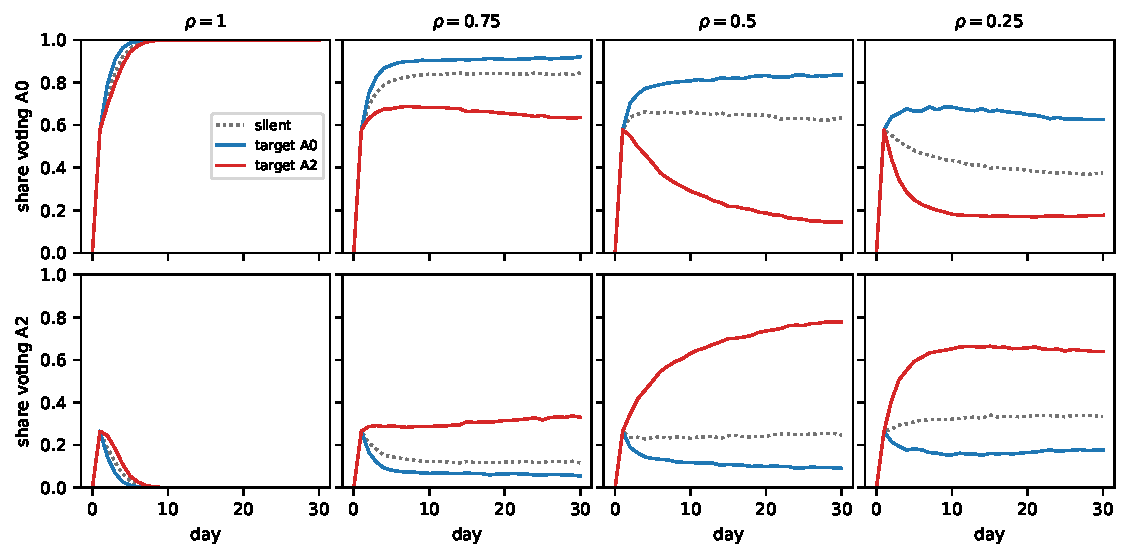
\includegraphics[width=0.95\linewidth]{figures/fig_votes.pdf}
\caption{Share of agents voting A0 (top) and A2 (bottom) at the end of each day, Eq.~(\ref{eq:share}), without a
controller (dotted), with the controller targeting A0 (blue) and A2 (red); one column per memory $\rho$. $q = 6$,
$q_c = 12$, $b = 1$, gate on. Day 0: nobody has voted yet, every share is 0. 95\% intervals are narrower than the
lines ($\pm 0.01$).}
\label{fig:votes}
\end{figure}

\begin{itemize}\itemsep1pt
\item \textbf{The shorter the memory, the less firmly the silent swarm holds the truth}: 100\%, 85\%, 63\% and
  38\% vote A0 on day 30 for $\rho = 1, 0.75, 0.5, 0.25$.
\item \textbf{With full memory no controller matters}: every agent votes A0 by day $\approx 8$ in all three arms.
\item \textbf{The false controller wins the majority when $\rho \le 0.5$}: A2 gets 78\% ($\rho = 0.5$) and 64\%
  ($\rho = 0.25$) of the votes, against 25\% and 33\% in silence; at $\rho = 0.75$ only 33\%.
\item \textbf{The truth controller restores the truth} to 92\% ($\rho = 0.75$) and 84\% ($\rho = 0.5$), but only to
  63\% at $\rho = 0.25$.
\end{itemize}

\section{Observables as time series}\label{sec:time}

\begin{figure}[H]
\centering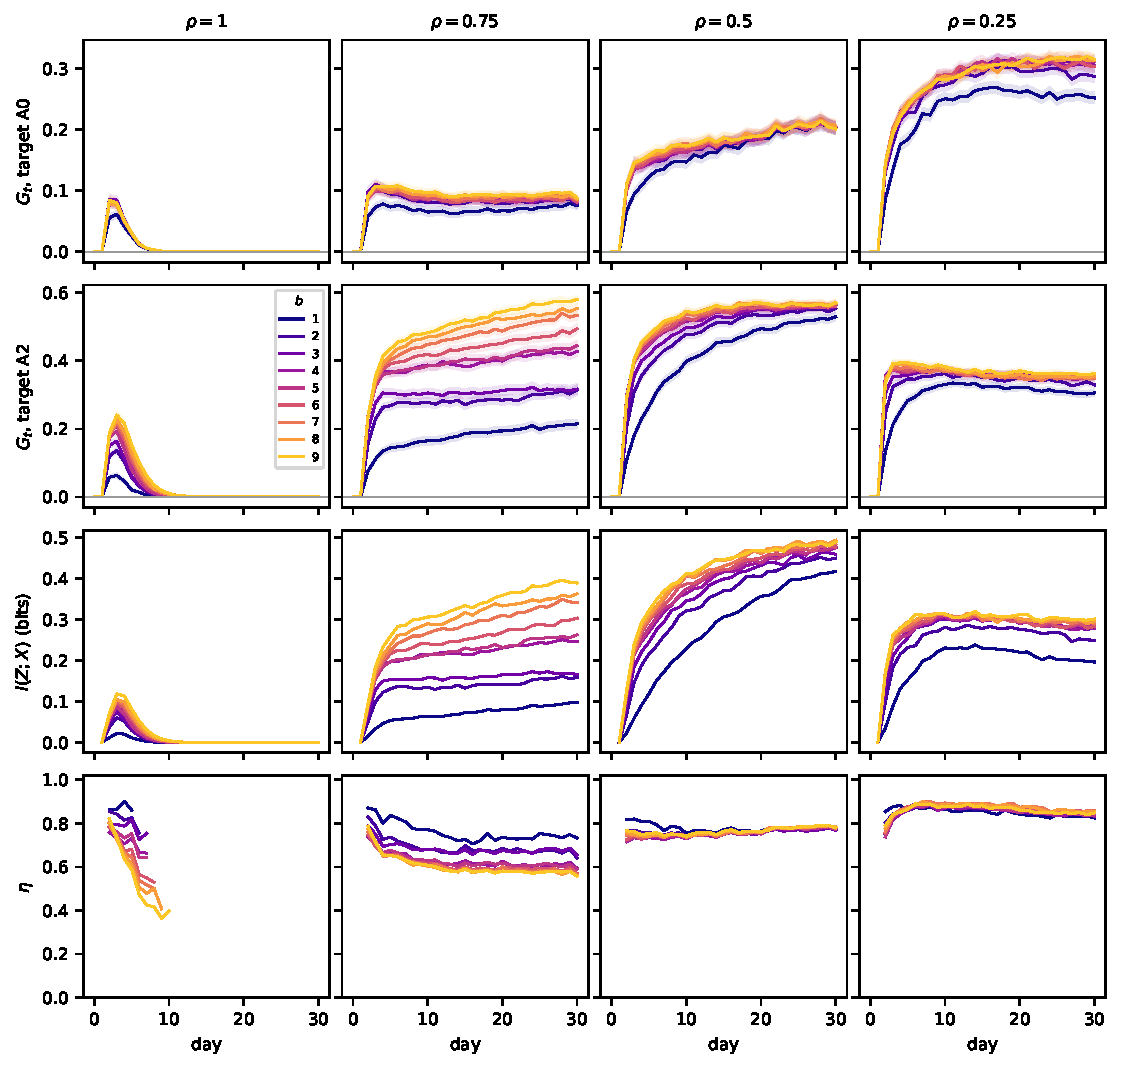
\includegraphics[width=0.95\linewidth]{figures/fig_timeseries.pdf}
\caption{All observables over the days, one column per memory $\rho$, one curve per budget $b$; $q = 6$,
$q_c = 12$, gate on. Rows: paired susceptibility $G_t$, Eq.~(\ref{eq:chi}), for target A0 and target A2 (bands:
95\% intervals; $G_0 = 0$); readability $I(Z;X)$, Eq.~(\ref{eq:I}); efficiency $\eta$, Eq.~(\ref{eq:eta}) (blank:
undefined).}
\label{fig:timeseries}
\end{figure}

\begin{figure}[H]
\centering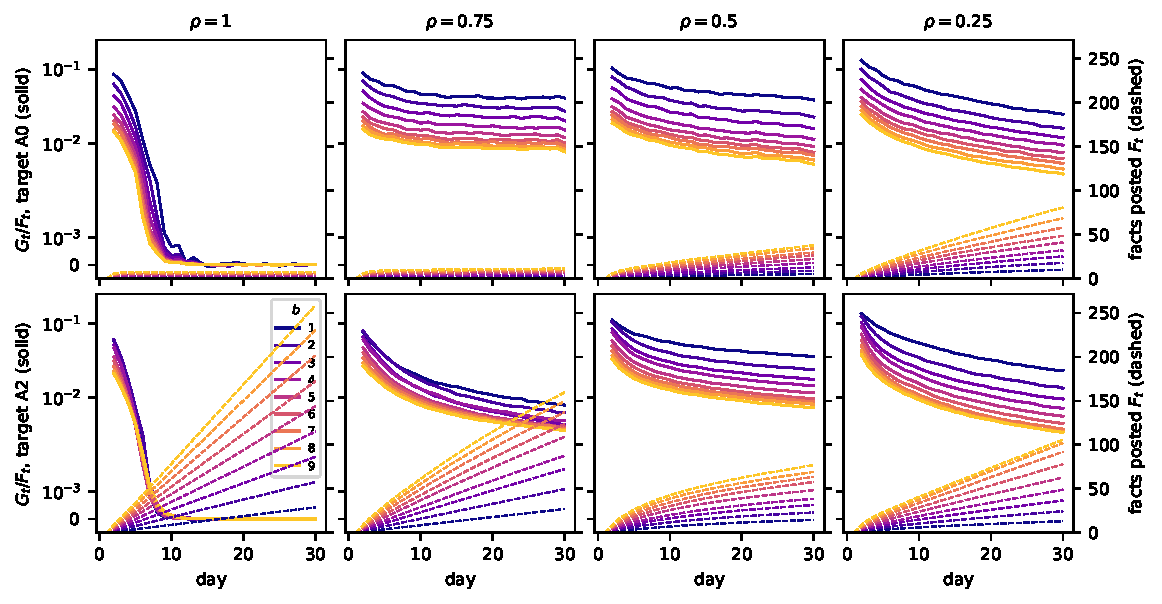
\includegraphics[width=0.95\linewidth]{figures/fig_per_fact.pdf}
\caption{Gain per fact $G_t/F_t$ (solid, left axis, log scale; shown once at least half a fact has been posted)
and facts posted $F_t$ (dashed, right axis), target A0 (top) and A2 (bottom), one colour per budget; $q = 6$,
$q_c = 12$, gate on.}
\label{fig:perfact}
\end{figure}

\paragraph{Susceptibility (Figure~\ref{fig:timeseries}, rows 1--2).}
\begin{itemize}\itemsep1pt
\item \textbf{It peaks at intermediate memory}: on day 30, target A2, $G = 0.22$--$0.58$ ($\rho = 0.75$),
  $0.53$--$0.57$ ($\rho = 0.5$), $0.31$--$0.36$ ($\rho = 0.25$); target A0, $0.08$--$0.09$, $0.20$,
  $0.25$--$0.32$.
\item \textbf{With full memory it is only transient}: target A2 reaches $0.24$ on day 3 ($b = 9$) and is gone by
  day $\approx 12$.
\item \textbf{The budget matters only when agents remember well}: at $\rho = 0.75$, target A2 grows from $0.22$
  ($b = 1$) to $0.58$ ($b = 9$); at $\rho \le 0.5$ every $b \ge 2$ gives about the same.
\item \textbf{With heavy forgetting a large budget overshoots}: at $\rho = 0.25$, $b = 9$, target A2 peaks at $0.39$
  (day 5) and settles at $0.36$.
\end{itemize}

\paragraph{Readability and efficiency (rows 3--4).}
\begin{itemize}\itemsep1pt
\item \textbf{Readability has the shape of the susceptibility}: it is largest at $\rho = 0.5$ ($I = 0.42$--$0.49$
  bits on day 30), grows with the budget at $\rho = 0.75$ ($0.10 \to 0.39$) and is transient with full memory.
\item \textbf{Efficiency moves much less}: after day 3, $\eta = 0.82$--$0.90$ ($\rho = 0.25$), $0.73$--$0.82$
  ($\rho = 0.5$), $0.56$--$0.86$ ($\rho = 0.75$). It falls with the budget only at $\rho = 0.75$, where the false
  controller grows with $b$ while the truth controller is near its ceiling: $\eta$ reports how symmetric the two
  controllers' effects are, not their size.
\end{itemize}

\paragraph{Gain per fact and facts posted (Figure~\ref{fig:perfact}).}
\begin{itemize}\itemsep1pt
\item \textbf{Each fact buys most in the first days}: $G_t/F_t$ is largest early and falls as facts accumulate.
\item \textbf{The smallest budget is the most effective per fact}: on day 30, target A2, $\rho = 0.5$: $0.036$ per
  fact at $b = 1$ (15 facts) against $0.007$ at $b = 9$ (77 facts); at $\rho = 0.25$: $0.023$ against $0.003$.
\item \textbf{The facts posted grow almost linearly with $b$ for the false controller} (up to 160 by day 30 at
  $\rho = 0.75$); the truth controller posts only 2--81, because the gate keeps it silent once the swarm agrees,
  which is why it gets more per fact ($0.039$ at $\rho = 0.5$, $b = 1$).
\end{itemize}

\section{Phase diagrams}\label{sec:phase}

All panels on day 30, gate on; the susceptibility is for target A2 (grey number: its 95\% interval includes 0);
readability and efficiency are for the pair of targets. Colour scales are shared with the Simulation 2 report.

\begin{figure}[H]
\centering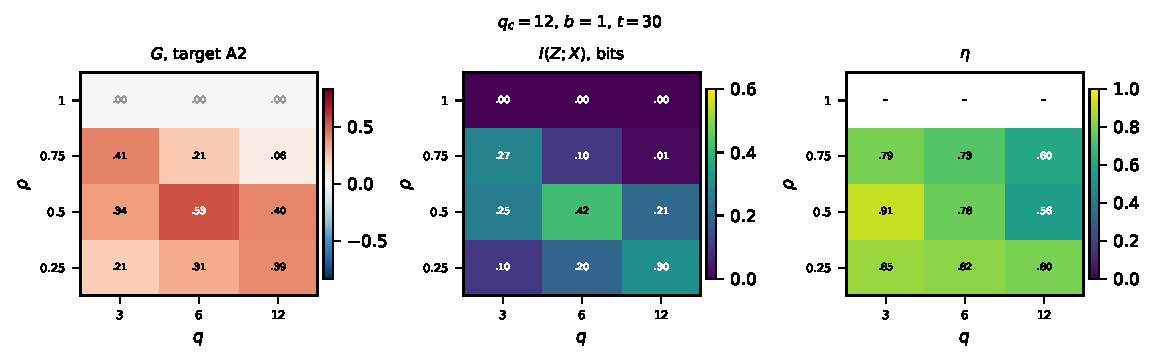
\includegraphics[width=0.98\linewidth]{figures/fig_phase_rho_q.pdf}
\caption{Susceptibility, readability and efficiency over memory $\rho$ and the posts each agent reads $q$;
$q_c = 12$, $b = 1$.}
\label{fig:phaserq}
\end{figure}

\begin{itemize}\itemsep1pt
\item \textbf{Reading more defends the proof only when agents remember well}: at $\rho = 0.75$, $G$ falls from
  $0.41$ ($q = 3$) to $0.06$ ($q = 12$) and $I$ from $0.27$ to $0.01$ bits; at $\rho = 0.25$, $G$ rises from $0.21$ to
  $0.40$ and $I$ from $0.10$ to $0.30$. A likely reason, not tested: with heavy forgetting the proof cannot be rebuilt
  anyway, and reading more only spreads the controller's facts faster.
\item \textbf{$\eta$ stays at 0.56--0.91}, unrelated to this reversal.
\end{itemize}

\begin{figure}[H]
\centering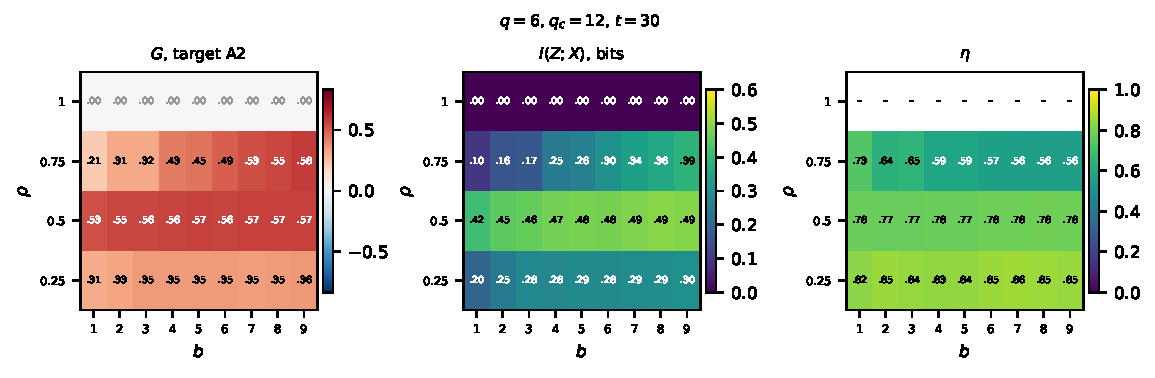
\includegraphics[width=0.98\linewidth]{figures/fig_phase_rho_x.pdf}
\caption{Susceptibility, readability and efficiency over memory $\rho$ and the budget $b$; $q = 6$, $q_c = 12$.}
\label{fig:phaserx}
\end{figure}

\begin{itemize}\itemsep1pt
\item \textbf{Memory sets the level}: $G = 0$ at $\rho = 1$, largest at $\rho = 0.5$ (0.53--0.57); the budget
  matters only at $\rho = 0.75$ (0.22 to 0.58).
\item \textbf{$G$ and $I$ move together} ($I$ from $0.10$ to $0.49$ bits); \textbf{$\eta$ moves the other way at
  $\rho = 0.75$} (0.73 to 0.56 as $b$ grows), where the pair turns lopsided.
\end{itemize}

\begin{figure}[H]
\centering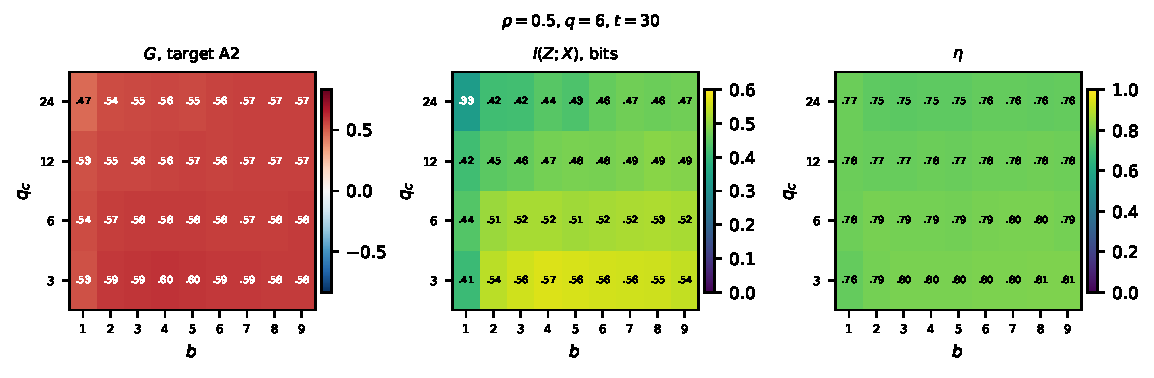
\includegraphics[width=0.98\linewidth]{figures/fig_phase_qc_x.pdf}
\caption{Susceptibility, readability and efficiency over the posts the controller reads $q_c$ and the budget $b$;
$\rho = 0.5$, $q = 6$.}
\label{fig:phaseqx}
\end{figure}

\begin{itemize}\itemsep1pt
\item \textbf{At $\rho = 0.5$ neither the controller's reading nor its budget matters much}: $G = 0.47$--$0.60$
  (mean $0.58$, $0.57$, $0.56$, $0.55$ for $q_c = 3, 6, 12, 24$); $I = 0.33$--$0.57$ bits; $\eta = 0.75$--$0.81$.
\item \textbf{Reading fewer posts helps slightly}, likely because with few posts read the vote gate silences the
  controller less often (not checked).
\end{itemize}

\section{Susceptibility against the budget, and its slope}\label{sec:strength}

\begin{figure}[H]
\centering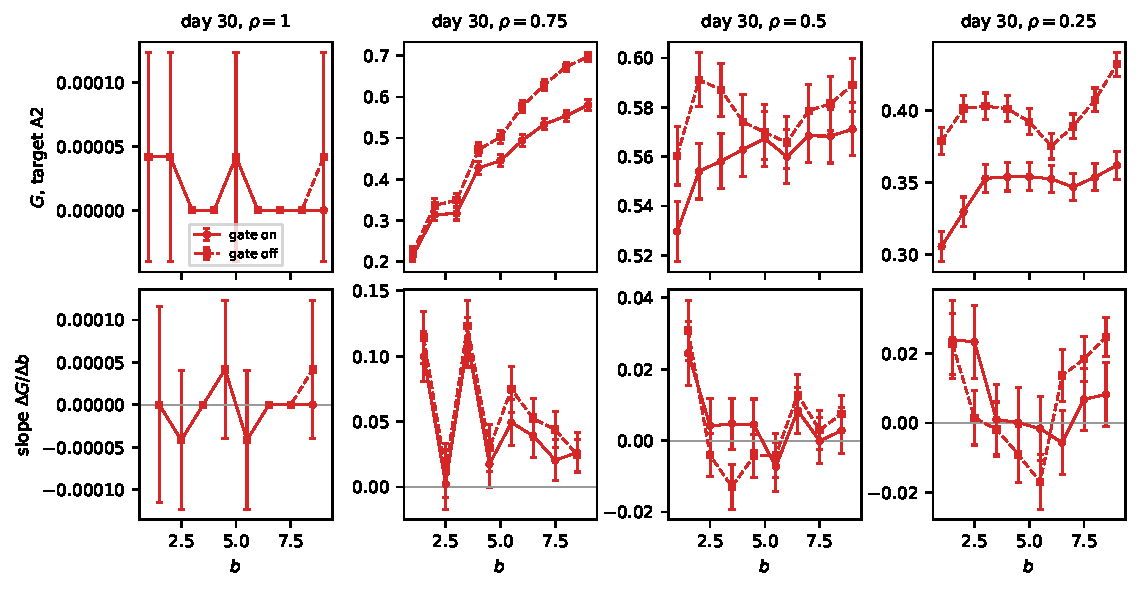
\includegraphics[width=0.95\linewidth]{figures/fig_gain_strength.pdf}
\caption{Top: $G$ on day 30, target A2, against the budget $b$, one panel per $\rho$; gate on (solid) and off
(dashed); bars: 95\% intervals. Bottom: the slope between neighbouring budgets, Eq.~(\ref{eq:slope}), with paired 95\% intervals.}
\label{fig:strength}
\end{figure}

\begin{figure}[H]
\centering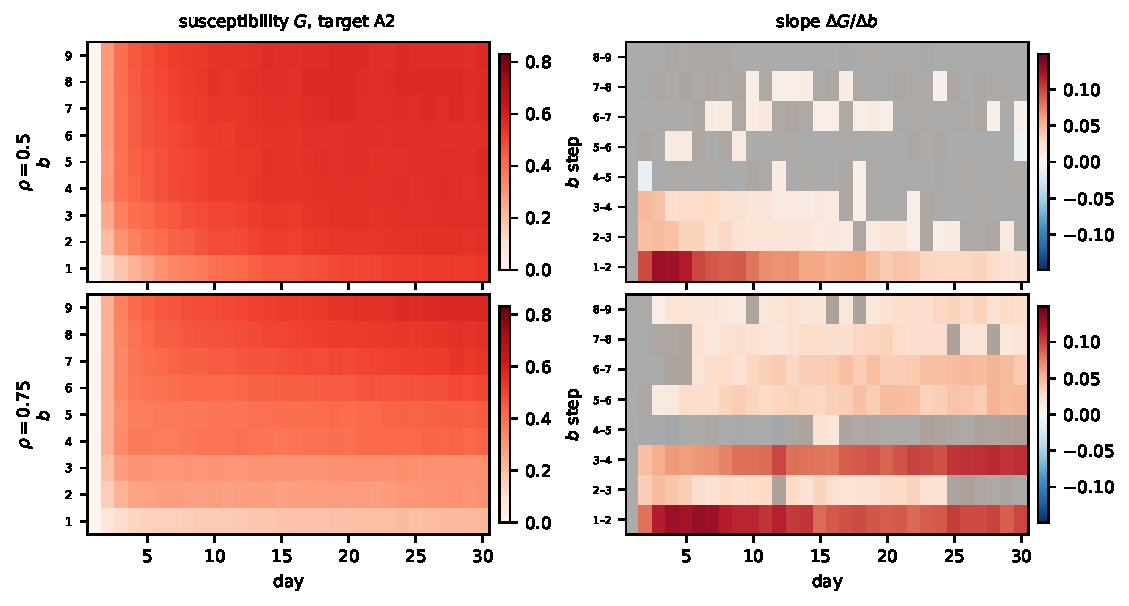
\includegraphics[width=0.95\linewidth]{figures/fig_strength_time.pdf}
\caption{$G$, target A2 (left), and its slope between neighbouring budgets (right) over the days ($x$) and the
budget ($y$), for $\rho = 0.5$ (top) and $0.75$ (bottom); $q = 6$, $q_c = 12$, gate on. Each row of the right panels
is one step between neighbouring budgets; faded cells: its paired 95\% interval includes 0.}
\label{fig:strengthtime}
\end{figure}

\begin{itemize}\itemsep1pt
\item \textbf{When agents remember well, more budget keeps buying susceptibility} (Figure~\ref{fig:strength}): at
  $\rho = 0.75$ the slope is $0.10$ for the first step and still $0.04$ on average after it; at $\rho = 0.5$ and
  $0.25$ it is $0.02$ for the first step and about $0.002$ after it.
\item \textbf{At $\rho = 0.5$ the slope fades with time} (Figure~\ref{fig:strengthtime}): the first step falls from
  $0.12$ (day 5) to $0.02$ (day 30) as $b = 1$ catches up; $b = 9$ reaches 90\% of its day-30 value by day 7, $b = 1$
  by day 19.
\item \textbf{At $\rho = 0.75$ it does not}: on day 30 most steps are still significantly positive ($b = 1 \to 2$:
  $0.10$; $3 \to 4$: $0.11$; $5 \to 9$: $0.02$--$0.05$), and the step from $b = 3$ to 4 grows from $0.05$ (day 2) to
  $0.11$ (day 30). More budget pays more the longer control lasts.
\item \textbf{The returns come in uneven steps}: at $\rho = 0.75$ the steps $2 \to 3$ and $4 \to 5$ add nothing
  measurable while their neighbours add $0.05$--$0.11$. A likely reason, not tested: the best set of $b$ facts from the
  12-fact pool changes composition only at some values of $b$.
\item \textbf{Turning the gate off adds susceptibility where the budget matters}: up to $+0.12$ at $\rho = 0.75$.
\end{itemize}

\section{Who holds the proof}

\begin{figure}[H]
\centering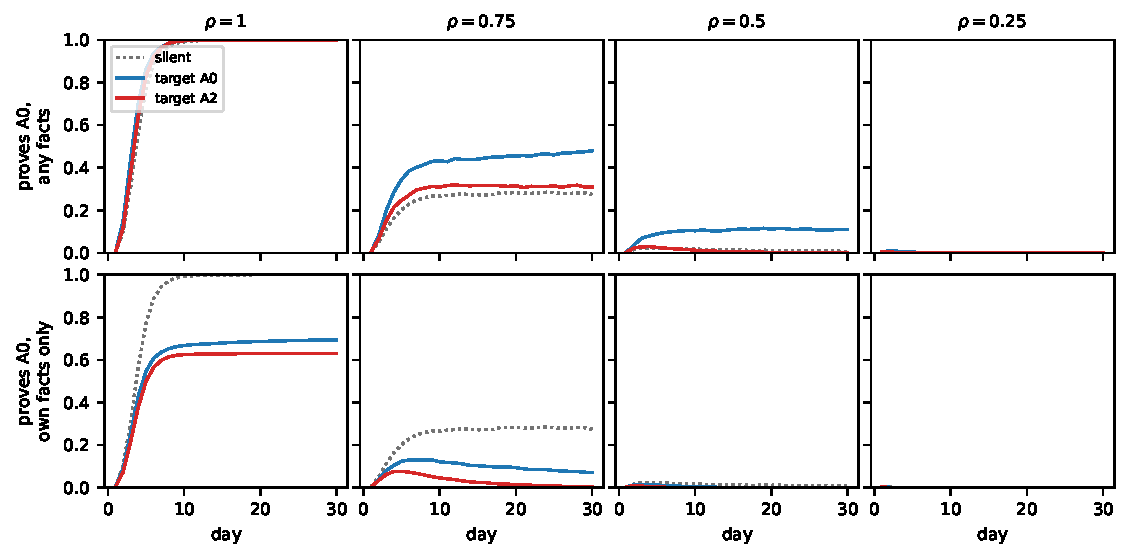
\includegraphics[width=0.95\linewidth]{figures/fig_proofs.pdf}
\caption{Share of agents whose remembered facts prove A0 (top) and prove it from the agents' original facts only
(bottom); silent (dotted), target A0 (blue), target A2 (red); $q = 6$, $q_c = 12$, $b = 1$, gate on.}
\label{fig:proofs}
\end{figure}

\begin{itemize}\itemsep1pt
\item \textbf{Proofs need memory}: on day 30 the silent swarm has 100\%, 28\%, 1\% and 0\% of agents proving A0
  for $\rho = 1, 0.75, 0.5, 0.25$. Below $\rho = 0.75$ votes rest on beliefs, not proofs.
\item \textbf{Every controller replaces the agents' own proofs}: with full memory all agents prove A0 under any
  arm, but only 69\% (target A0) and 63\% (target A2) from their own facts (100\% in silence); at $\rho = 0.75$,
  48\% prove A0 under the truth controller but only 7\% from their own facts.
\item \textbf{The false controller's true facts complete proofs of A0} (31\% against 28\% in silence at
  $\rho = 0.75$), while own-evidence proofs fall to 0.5\%.
\end{itemize}

\section{Conclusions}

\begin{enumerate}\itemsep2pt
\item \textbf{Memory decides whether a swarm that owns a proof can be steered.} With full memory every effect
  vanishes within about ten days. As memory shortens the silent swarm holds the truth less firmly (100\%, 85\%, 63\%,
  38\% voting A0 on day 30), and the susceptibility peaks at $\rho = 0.5$.
\item \textbf{Susceptibility and readability move together; efficiency does not.} In every time series and phase
  diagram $G$ and $I$ rise, fall and reverse together; $\eta$ stays at 0.56--0.91 and falls only where one controller
  grows much more than the other.
\item \textbf{More budget pays only when agents remember well}, and there it pays more the longer control lasts;
  elsewhere one fact per night is almost enough and the most effective per fact.
\item \textbf{The posts each agent reads switch sides with memory}: they defend the proof at $\rho = 0.75$ and help
  the controller at $\rho = 0.25$, in susceptibility and readability alike.
\item \textbf{Control replaces the agents' own proofs}, even when every agent ends up proving the truth.
\item \textbf{Compared with Simulation 2} (same settings, about the same facts posted): Simulation 1 is more
  susceptible at $\rho = 0.5$ (0.53 against 0.33, target A2) and less at $\rho = 0.25$ (0.31 against 0.43).
\end{enumerate}

\paragraph{Caveats.} One world, 24 exact-Bayesian agents voting by probability matching, one controller policy
posting a fixed batch each night; 1{,}000 episodes per setting (95\% intervals on $G$ about $\pm0.02$). Information
is plug-in from 1{,}000 episodes per arm. Data:
\texttt{results/simulation\_1/2026-10-15\_sim1\_pm\_symmetric\_fine}; tables and figures:
\texttt{analysis/task003\_llm\_free/shared\_analysis/gold\_standard/}.

\end{document}
